\documentclass[a4paper,11pt]{article}
\usepackage{lecturenotes}
\usepackage{multicol}
\usepackage{scrextend}

\lectureheader{ELE734}{1}
\begin{document}
\tableofcontents
\clearpage
\notesection{MOS Devices}
\notedefinition{Feature Size}{Channel length of a MOSFET}
\begin{figure}[htbp]
    \centering
    \begin{minipage}[t]{0.48\linewidth}
        \centering
        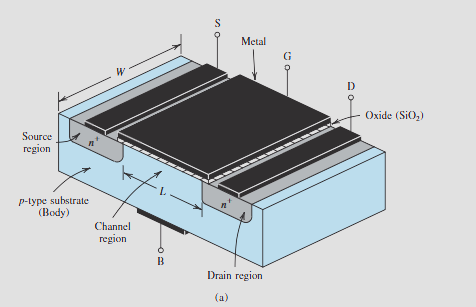
\includegraphics[height=4cm]{figures/nmos-device-structure.png}
        \caption{NMOS Device Structure}
        \label{fig:NMOS-Device-Structure}
    \end{minipage}\hfill
    \begin{minipage}[t]{0.48\linewidth}
        \centering
        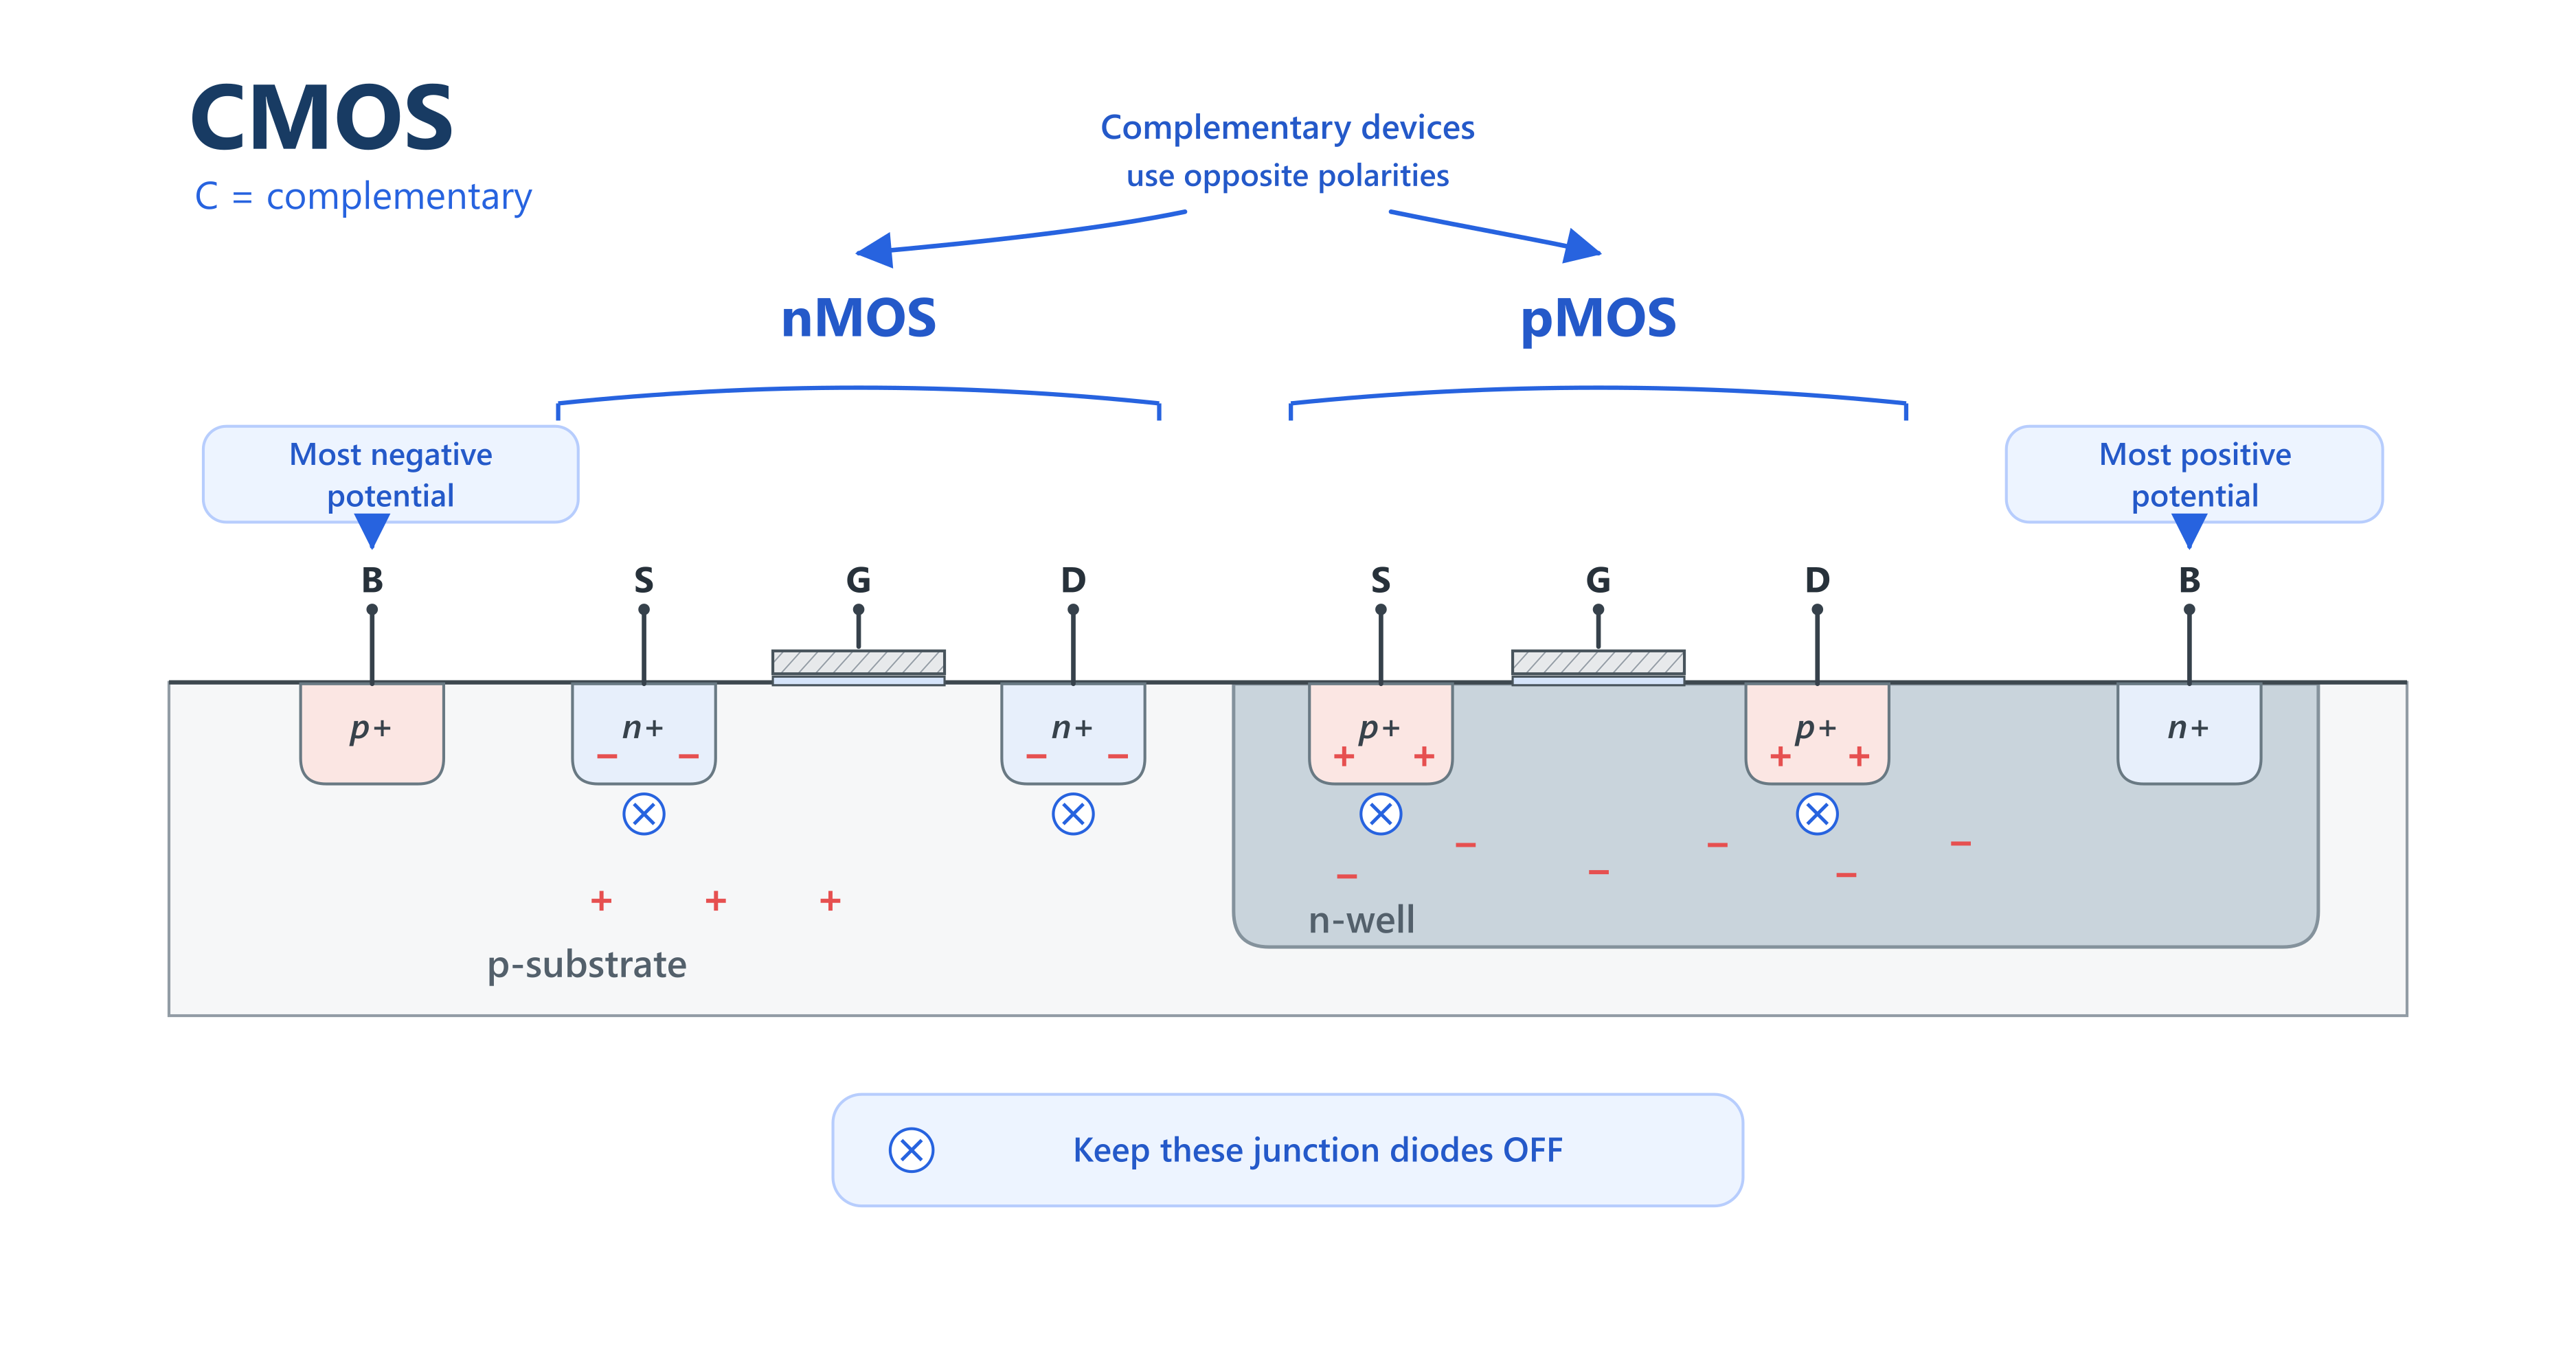
\includegraphics[height=4cm]{figures/cmos-device-annotated.png}
        \caption{CMOS Device Structure}
        \label{fig:CMOS-Device-Structure}
    \end{minipage}
\end{figure}


CMOS devices combine both NMOS and PMOS into a single device.

\begin{notecircuit}[scale=0.5, transform shape]{CMOS Device}
    \draw (0, 1) node[pmos, arrowmos] (pmos) {$M_1$};
    \draw (0, -1) node[nmos, arrowmos] (nmos) {$M_2$};

    \draw(pmos.drain) -- (nmos.drain) coordinate[midway] (out);
    \node[right] at (out) {$Y$};

    \draw(pmos.gate) -- (nmos.gate) coordinate[midway] (in);
    \node [left] at (in) {$A$};

    \draw(pmos.source) -- ++(0,0.8) node[vcc] {$V_{DD}$};
    \draw (nmos.source) -- ++(0,-0.8) node[ground] {};
\end{notecircuit}

\subnotesection{CMOS vs. PMOS or NMOS}
\begin{itemize}
    \item[-] \textbf{PMOS} is more difficult to build
          \begin{itemize}
              \item In Planar layout, PMOS is only $\frac{1}{2}$ as fast as NMOS
              \item Brings no new functionalities vs. NMOS
          \end{itemize}
    \item[-] \textbf{NMOS} on the other hand has high static power consumption
          \begin{itemize}
              \item NMOS provides direct path from $S \rightarrow GND$ when it is on. Therefore it is not a perfect switch, and cannot pull voltage all the way to $V_{DD}$
          \end{itemize}
\end{itemize}

\notedefinition{PMOS \& NMOS Pros and Cons}{
    A PMOS device is \textbf{half the speed} as a NMOS device, and cannot pull voltage all the way \textbf{DOWN} to GND. \\ \hfill \break
    A NMOS device is not a perfect switch, and cannot pull voltage all the way \textbf{UP} to $V_{DD}$
}

\notesection{Pass Transistor Style and Transmission Gate Style}
A pass transistor style only uses NMOS devices and is commonly found in FPGA's. A transmission gate design style can use both NMOS and PMOS devices.
\subnotesection{Pass Transistor Style}

\begin{figure}[htbp]
    \centering
    \begin{minipage}[t]{0.48\linewidth}
        \centering
        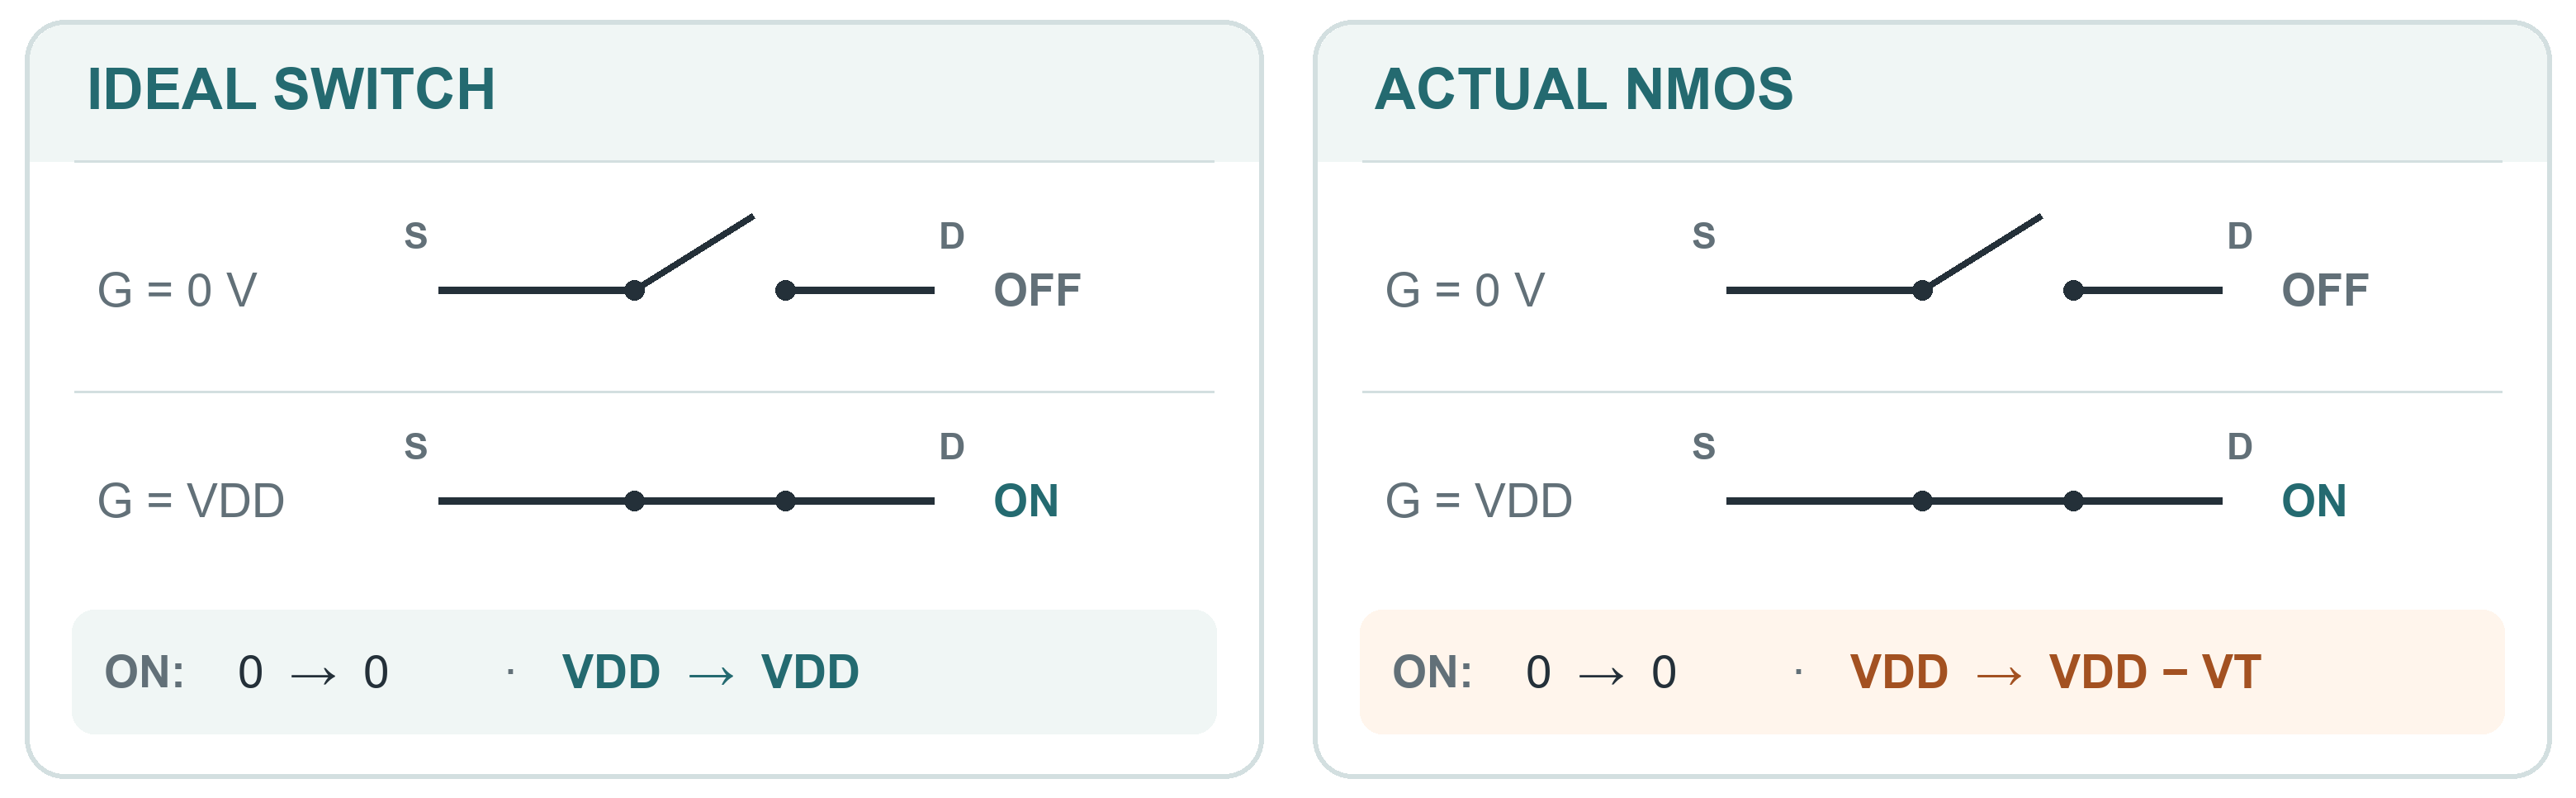
\includegraphics[width=\linewidth]{figures/nmos-pass-transistor-ideal-vs-actual.png}
        \caption{Ideal Pass Transistor vs. Non Ideal}
        \label{fig:pass-transistor-ideal-vs-actual}
    \end{minipage}\hfill
    \begin{minipage}[t]{0.48\linewidth}
        \centering
        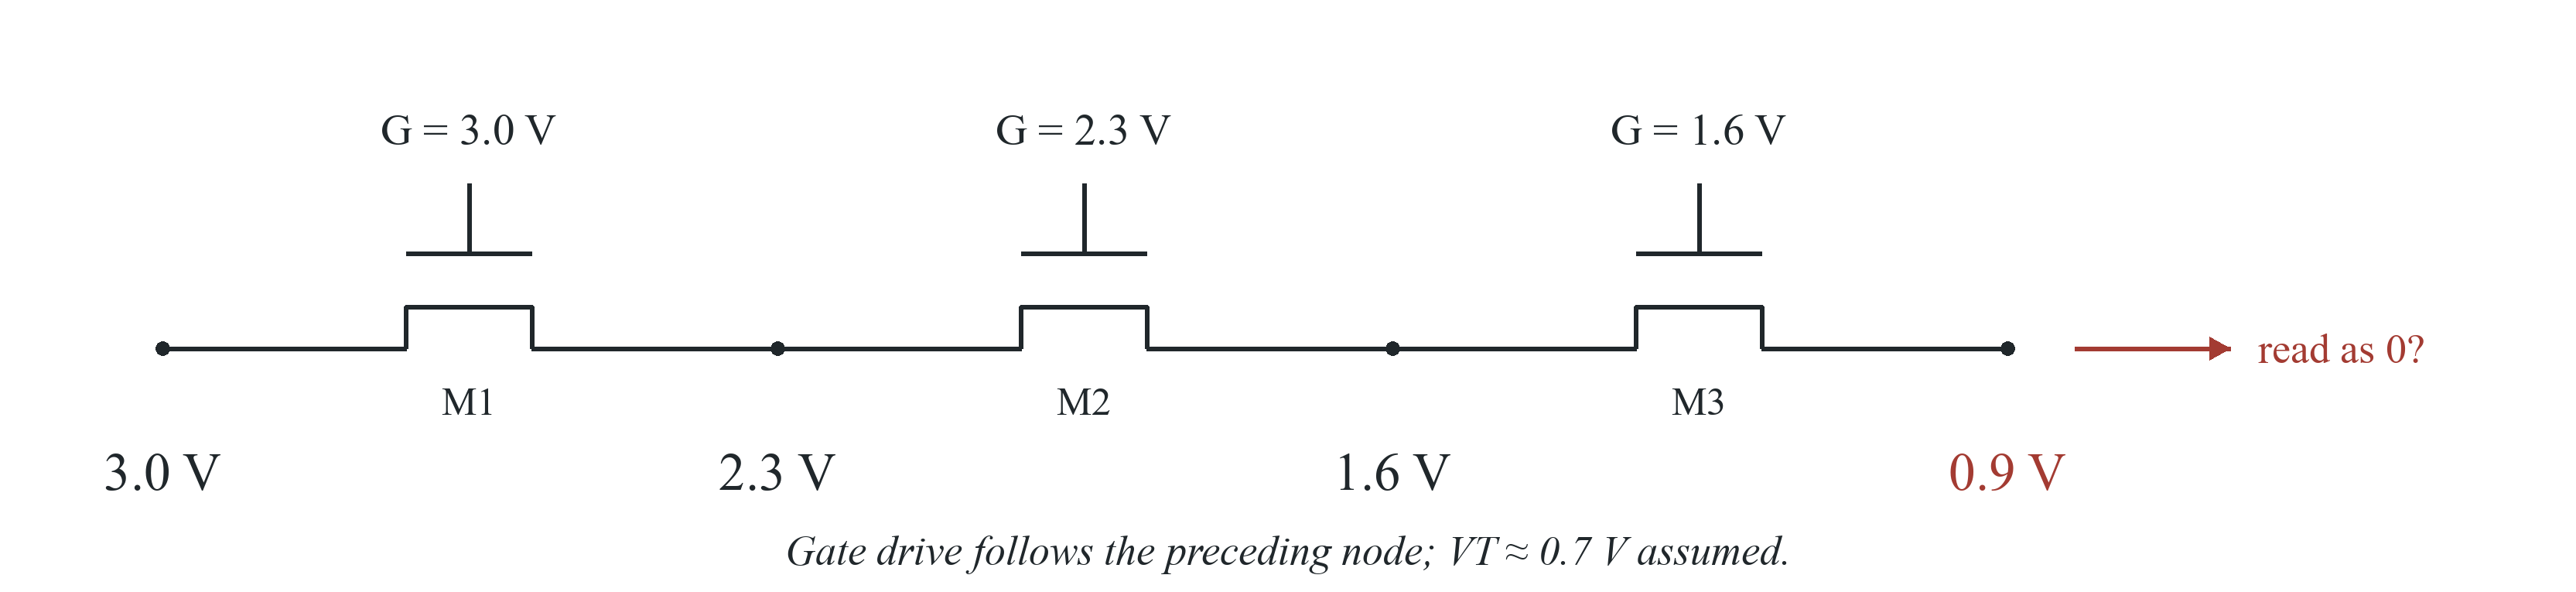
\includegraphics[width=\linewidth]{figures/nmos-pass-chain-no-restoration.png}
        \caption{Con of Pass Transistor Non-ideal Behaviour}
        \label{fig:chain-pass-no-res}
    \end{minipage}
\end{figure}

\notedefinition{Pass Transmission Summary}{
    Boosting is needed to increase gate voltage such that it is 1 threshhold voltage higher than normal $V_{DD}$.
    \par\vspace{10pt}
    \begin{tabularx}{\linewidth}{@{}>{\color{NoteMuted}}l@{\hspace{1em}}X@{}}
        Pro  & Only uses NMOS to do computation                             \\[4pt]
        Cost & Requires the use of an additional power distribution network
    \end{tabularx}
}

\subnotesection{Transmission Gate Style}

Below is a figure demonstrating how a transmission gate style looks like:
\begin{figure}[htbp]
    \centering
    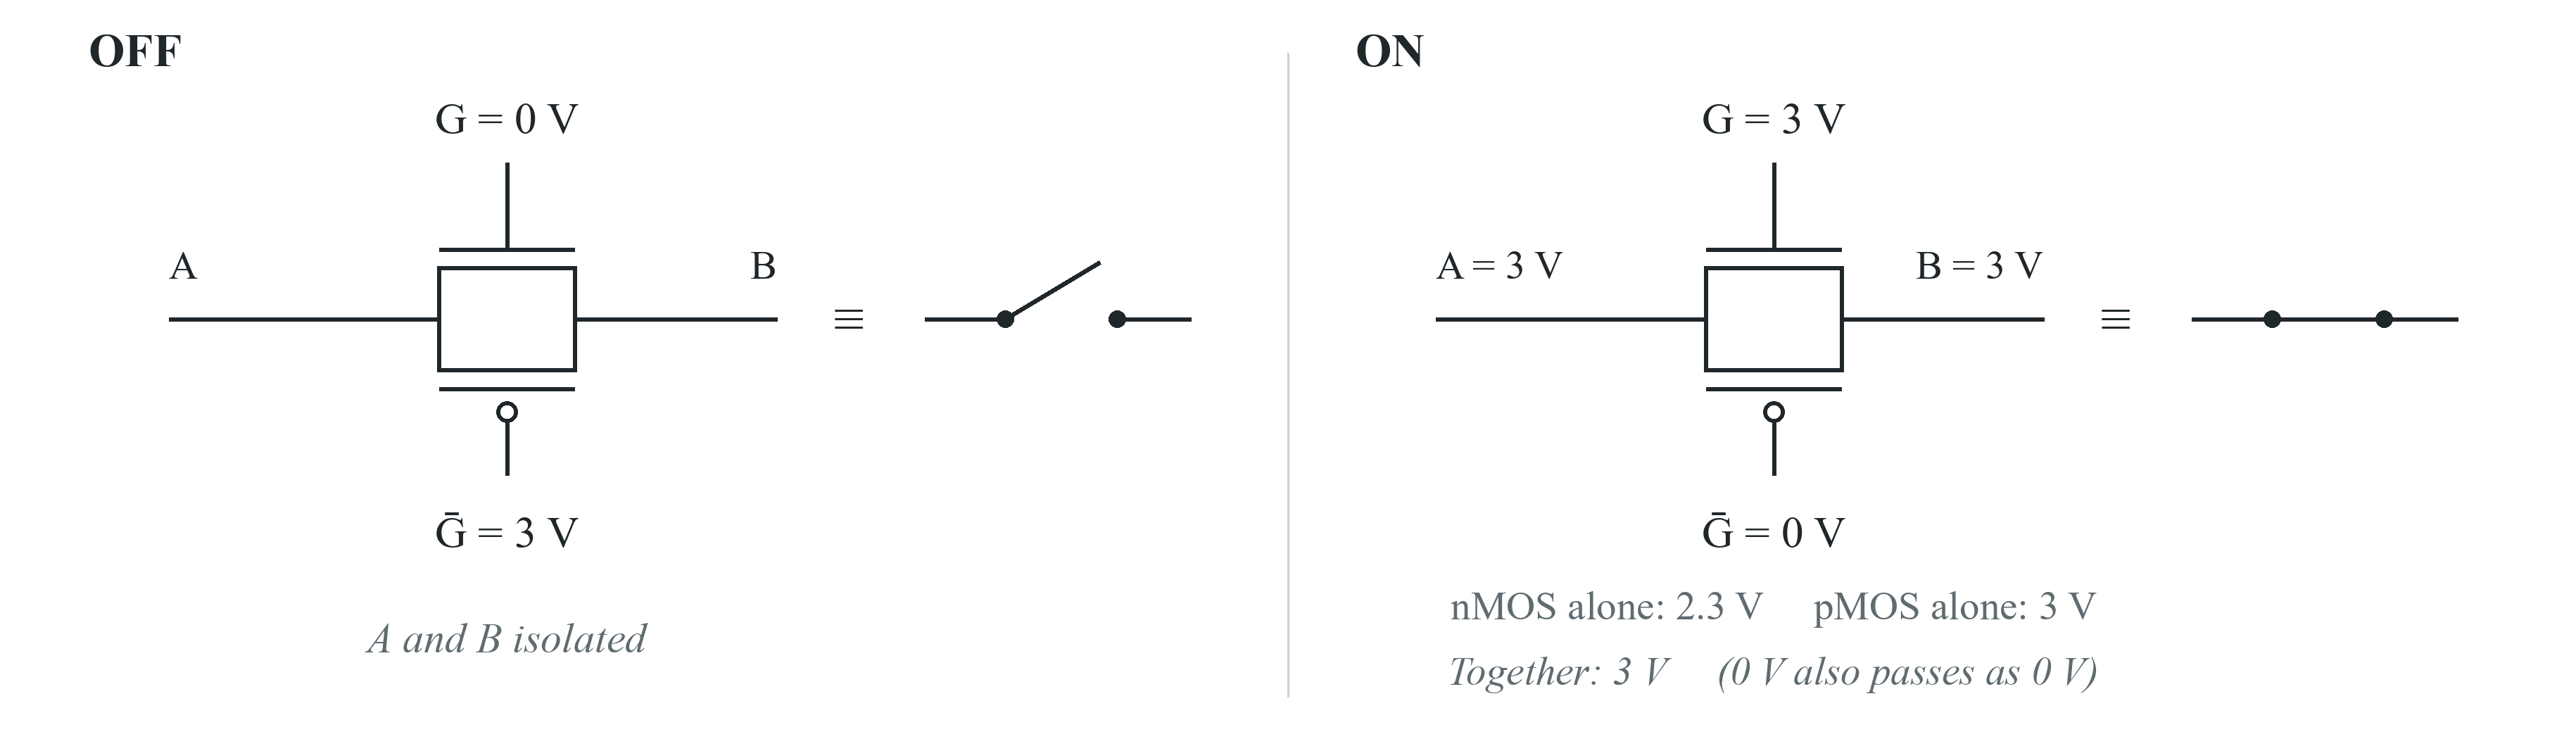
\includegraphics[width=0.8\linewidth]{figures/transmission-gate-off-on.png}
    \caption{Transmission Gate in Off and On State}
    \label{fig:trans-gate-in-and-on}
\end{figure}

When the transmission gate is in the ON state, the NMOS contributes: $V_{in} - V_{th}$ to the output whilst the PMOS contributes the full $V_{in}$.
\notedefinition{Gate Trasmission Style Summary}{
    Whilst it does not have the same downfall as the pass transmission style, it costs \textbf{doubles the size}
}


\notesection{CMOS Inverter}
\vspace{-4pt}
\noindent
\begingroup
\centering
\begin{minipage}[t]{0.25\linewidth}
    \begin{notecircuit}[scale=0.56, transform shape]{CMOS Inverter}
        \draw (0,0.75) node[pmos, arrowmos] (inv-pmos) {};
        \draw (0,-0.75) node[nmos, arrowmos] (inv-nmos) {};

        \draw (inv-pmos.drain) -- (inv-nmos.drain) coordinate[midway] (inv-out);
        \draw (inv-pmos.gate) -- (inv-nmos.gate) coordinate[midway] (inv-in);
        \draw (inv-in) -- ++(-1.6,0) coordinate (inv-in-end)
        node[left] {$\mathrm{in}$};
        \draw (inv-out) -- ++(1.6,0) coordinate (inv-out-end)
        node[right] {$\mathrm{out}$};

        \node[above, color=NoteAccent] at (-1.25,0) {$0$};
        \node[below, color=red!75!black] at (-1.25,0) {$1$};
        \node[above, color=NoteAccent] at (1.25,0) {$1$};
        \node[below, color=red!75!black] at (1.25,0) {$0$};

        \draw (inv-pmos.source) -- ++(0,0.45) node[vcc] {$3\,\mathrm{V}$};
        \draw (inv-nmos.source) -- ++(0,-0.45) node[ground] {};
        \node at (0,-2.75) {\texttt{out = !in}};
    \end{notecircuit}
\end{minipage}\hfill
\begin{minipage}[t]{0.42\linewidth}
    \begin{notecircuit}[scale=0.56, transform shape]{CMOS buffer $\Rightarrow$ 2 inverter}
        \draw (-1.2,0.75) node[pmos, arrowmos] (buf-pmos-1) {};
        \draw (-1.2,-0.75) node[nmos, arrowmos] (buf-nmos-1) {};
        \draw (1.2,0.75) node[pmos, arrowmos] (buf-pmos-2) {};
        \draw (1.2,-0.75) node[nmos, arrowmos] (buf-nmos-2) {};

        \draw (buf-pmos-1.drain) -- (buf-nmos-1.drain) coordinate[midway] (buf-mid);
        \draw (buf-pmos-1.gate) -- (buf-nmos-1.gate) coordinate[midway] (buf-in-1);
        \draw (buf-pmos-2.drain) -- (buf-nmos-2.drain) coordinate[midway] (buf-out);
        \draw (buf-pmos-2.gate) -- (buf-nmos-2.gate) coordinate[midway] (buf-in-2);

        \draw (buf-in-1) -- ++(-1.15,0) coordinate (buf-in-end)
        node[left] {$\mathrm{in}$};
        \draw (buf-mid) -- (buf-in-2);
        \draw (buf-out) -- ++(1.15,0) coordinate (buf-out-end)
        node[right] {$\mathrm{out}$};

        \node[above, color=NoteAccent] at (-2.55,0) {$0$};
        \node[below, color=red!75!black] at (-2.55,0) {$1$};
        \node[above, color=NoteAccent] at (0,0) {$1$};
        \node[below, color=red!75!black] at (0,0) {$0$};
        \node[above, color=NoteAccent] at (2.1,0) {$0$};
        \node[below, color=red!75!black] at (2.1,0) {$1$};

        \draw (buf-pmos-1.source) -- ++(0,0.45) node[vcc] {$3\,\mathrm{V}$};
        \draw (buf-nmos-1.source) -- ++(0,-0.45) node[ground] {};
        \draw (buf-pmos-2.source) -- ++(0,0.45) node[vcc] {$3\,\mathrm{V}$};
        \draw (buf-nmos-2.source) -- ++(0,-0.45) node[ground] {};
        \node at (0,-2.75) {\texttt{out = in}};
    \end{notecircuit}
\end{minipage}\hfill
\begin{minipage}[t]{0.29\linewidth}
    \begin{notecircuit}[scale=0.54, transform shape]{bad buffer}
        \draw (0,0.75) node[nmos, arrowmos] (bad-nmos) {};
        \draw (0,-0.75) node[pmos, arrowmos] (bad-pmos) {};

        \draw (bad-nmos.source) -- (bad-pmos.source) coordinate[midway] (bad-out);
        \draw (bad-nmos.gate) -- (bad-pmos.gate) coordinate[midway] (bad-in);
        \draw (bad-in) -- ++(-1.5,0);
        \draw (bad-out) -- ++(2.1,0);

        \node[above, color=NoteAccent] at (-1.2,0) {$1$};
        \node[below, color=red!75!black] at (-1.2,0) {$0$};
        \node[anchor=west, color=NoteAccent] at (0.95,0.22) {$1\;(2.3\,\mathrm{V})$};
        \node[anchor=west, color=red!75!black] at (0.95,-0.22) {$0\;(0.7\,\mathrm{V})$};
        \node[color=NoteAccent] at (0.75,0.85) {\textsf{on}};
        \node[color=red!75!black] at (1.4,0.85) {\textsf{off}};
        \node[color=NoteAccent] at (0.75,-0.85) {\textsf{off}};
        \node[color=red!75!black] at (1.4,-0.85) {\textsf{on}};

        \draw (bad-nmos.drain) -- ++(0,0.45) node[vcc] {$3\,\mathrm{V}$};
        \draw (bad-pmos.drain) -- ++(0,-0.45) node[ground] {};
    \end{notecircuit}
\end{minipage}
\par
\endgroup

\notedefinition{Why Buffer?}{A buffer is useful since it re-generates the signal. It can be useful for driving loads (large capacitance) like along wire and the like}

\subnotesection{CMOS - Organization of its Networks}

\begin{figure}[htbp]
    \centering
    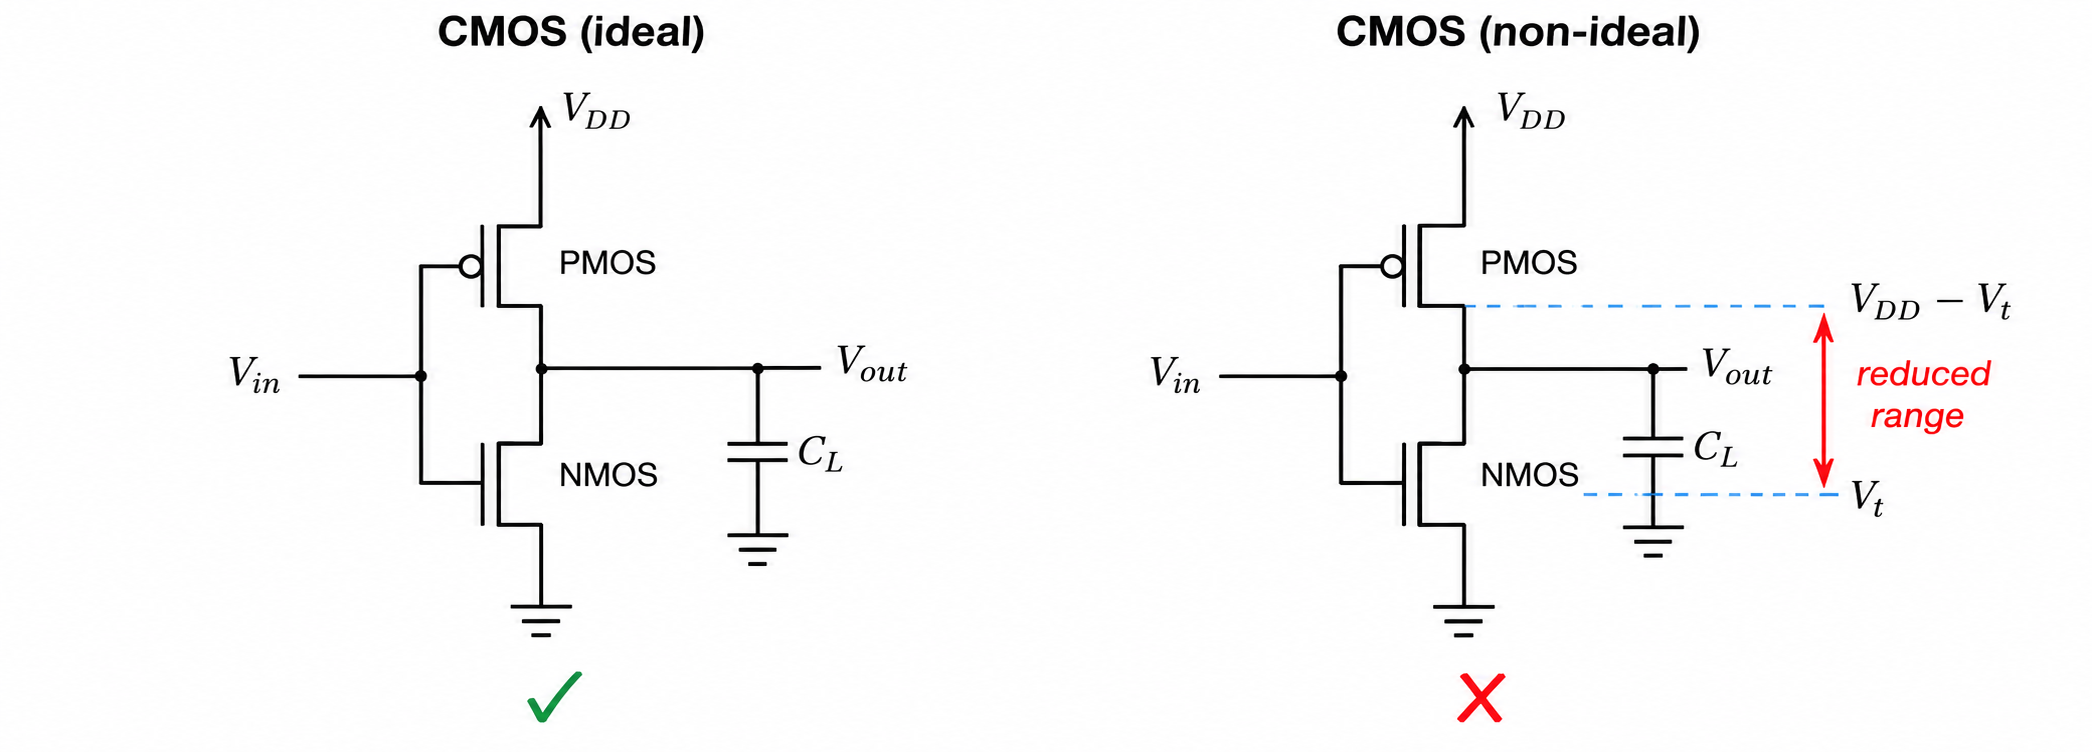
\includegraphics[width=0.8\linewidth]{figures/CMOS-network-organization.png}
    \caption{Why CMOS Circuits are Organized the Way they are}
    \label{fig:CMOS-network-organization}
\end{figure}

PMOS \textbf{must} be a complementary network of an NMOS. Meaning that the PMOS networks source must always be tied to $V_{DD}$ and the NMOS networks source must always be tied to $GND$.

\notebox{Complementary Networks}{
    \begin{itemize}
        \item PMOS is on $\Rightarrow$ NMOS must be off $\Rightarrow \text{output} = V_{DD}$
        \item NMOS is on $\Rightarrow$ PMOS must be off $\Rightarrow \text{output} = 0$
    \end{itemize}
}

\clearpage
\notesection{CMOS Logic Circuits}
CMOS logic consists of \textcolor{red}{Pull Up/Pull Down} networks, made of PMOS and NMOS transistors respectively.

\begin{figure}[htbp]
    \centering
    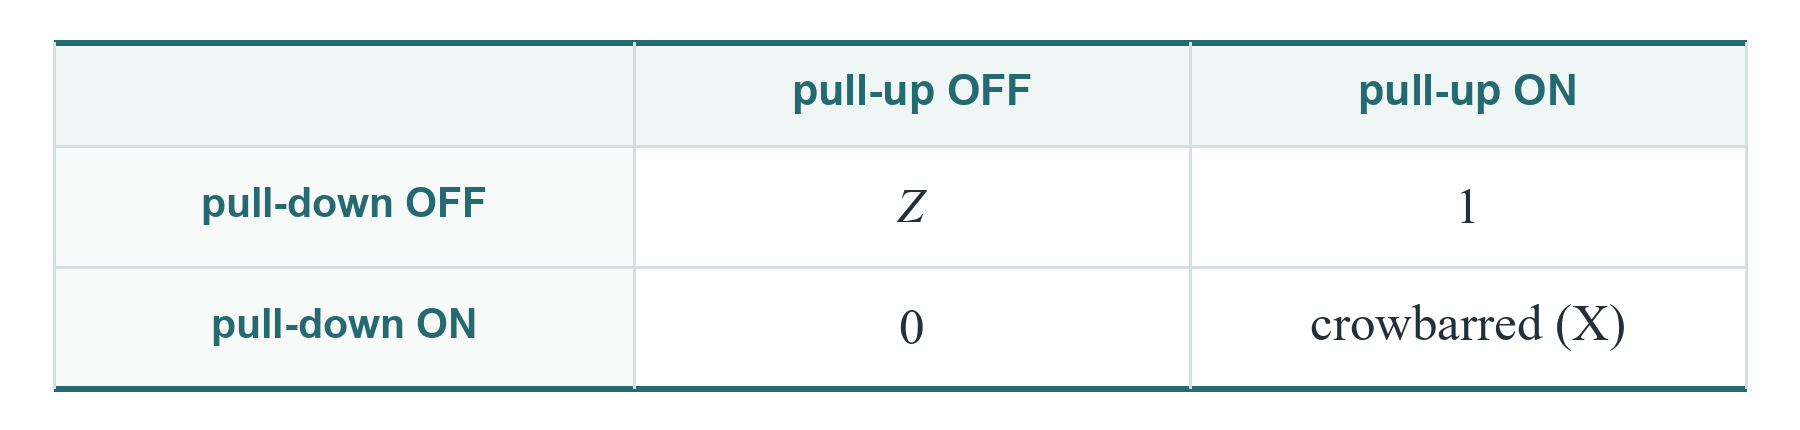
\includegraphics[width=0.82\linewidth]{figures/CMOS-output-states.png}
    \caption{Output states of CMOS logic gates}
    \label{fig:cmos-output-states}
\end{figure}

\notebox{Network notation}{
    \begin{tabularx}{\linewidth}{@{}>{\centering\arraybackslash}X!{\color{NoteRule}\vrule width 0.6pt}>{\centering\arraybackslash}X@{}}
        {\color{NoteAccent}\fontsize{28}{32}\selectfont\boldmath$+$}\par
        {\sffamily\bfseries\small Parallel}
         &
        {\color{NoteAccent}\fontsize{28}{32}\selectfont\boldmath$\cdot$}\par
        {\sffamily\bfseries\small Series}
    \end{tabularx}
}
\hfill \break
\textbf{Statements Regarding PDN/PUNs}
\begin{itemize}
    \item Series transistors are in a \textbf{ON} state if all of the transistors are ON
    \item Parallel transistors are in a \textbf{ON} state if any of the transistors are ON
    \item In general, when given a boolean expression, we want to find the expression s.t: $\bar{Y} = 0$.
          \begin{itemize}
              \item Consider $Y = \overline{A + B}$, to get the according CMOS expression, we simply evaluate  the expression for when $\bar{Y}$ is 0, which is simply the expression underneath the outer bar.
          \end{itemize}
\end{itemize}

\notedefinition{CMOS Gate Rule}{A basic CMOS gate is a naturally inverting operator. If the expression has an outer bar, i.e.
    $$
        Y = \overline{A\cdot B + C \cdot D}
    $$
    the expression underneath the outer bar is the PDN expression
}

\begin{figure}[htbp]
    \centering
    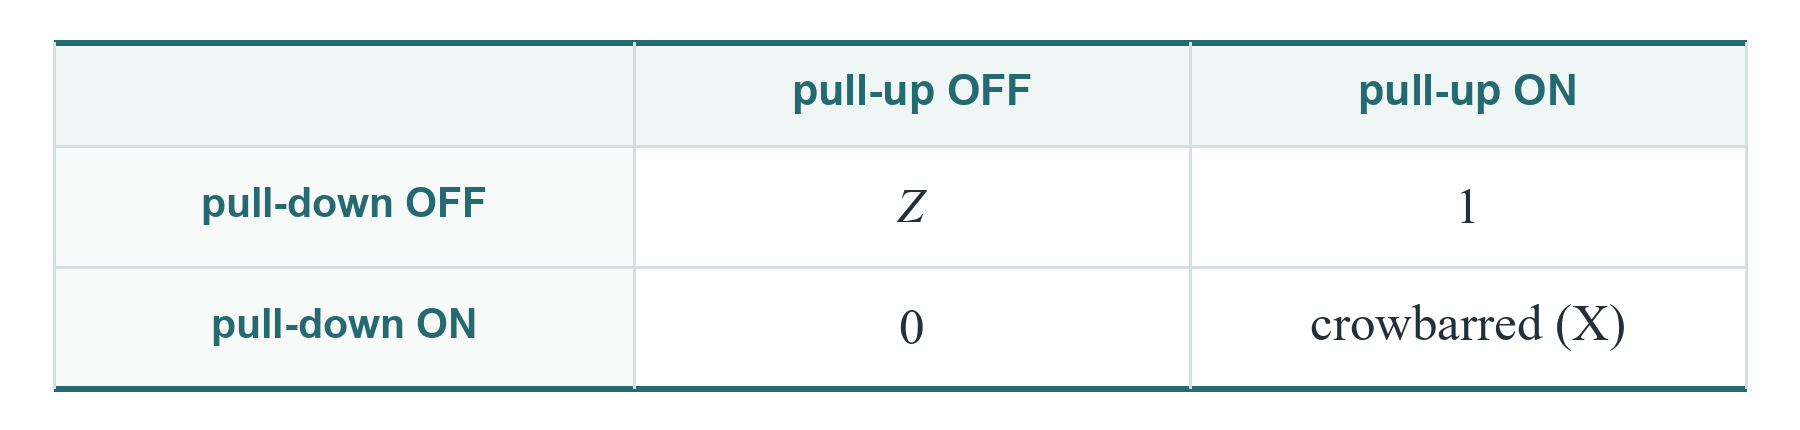
\includegraphics[width=0.8\linewidth]{figures/CMOS-output-states.png}
    \caption{CMOS Output States}
    \label{fig:CMOS-output-states}
\end{figure}


\begin{notetable}{XX}{\textbf{PDN} & \textbf{PUN}}
    Appear series in PDN & parallel in PUN \\
    Appear parallel in PDN & Series in PUN \\
\end{notetable}

\subnotesection{Inverter}

\noindent
\begin{minipage}[t]{0.46\linewidth}
    \begin{notecircuit}[scale=0.78, transform shape]{Digital logic symbol}
        \path[use as bounding box] (-2,-1.5) rectangle (2,1.5);
        \draw (0,0) node[not port] (logic-inverter) {};
        \draw (logic-inverter.in) -- ++(-1,0) node[left] {$A$};
        \draw (logic-inverter.out) -- ++(1,0) node[right] {$Y=\overline{A}$};
    \end{notecircuit}
\end{minipage}\hfill
\begin{minipage}[t]{0.52\linewidth}
    \begin{notecircuit}[scale=0.56, transform shape]{CMOS circuit}
        \draw (0,0.9) node[pmos, arrowmos] (logic-pmos) {};
        \draw (0,-0.9) node[nmos, arrowmos] (logic-nmos) {};

        \draw (logic-pmos.drain) -- (logic-nmos.drain) coordinate[midway] (logic-out);
        \draw (logic-pmos.gate) -- (logic-nmos.gate) coordinate[midway] (logic-in);
        \draw (logic-in) -- ++(-1.4,0) node[left] {$A$};
        \draw (logic-out) -- ++(2.3,0) node[right] {$Y$};

        \draw (logic-pmos.source) -- ++(0,0.45) node[vcc] {$V_{DD}$};
        \draw (logic-nmos.source) -- ++(0,-0.45) node[ground] {};
        \node[anchor=west, color=NoteAccent] at (0.55,0.9) {\textsf{Pull-up (PMOS)}};
        \node[anchor=west, color=NoteAccent] at (0.55,-0.9) {\textsf{Pull-down (NMOS)}};
    \end{notecircuit}
\end{minipage}
\par

\subnotesection{NAND Gate}
\noindent
\begin{minipage}[t]{0.27\linewidth}
    \begin{notecircuit}[scale=0.75, transform shape]{Digital logic symbol}
        \path[use as bounding box] (-1.8,-2.5) rectangle (1.8,2.5);
        \draw (0,0) node[nand port] (nand-symbol) {};
        \draw (nand-symbol.in 1) -- ++(-0.7,0) node[left] {$A$};
        \draw (nand-symbol.in 2) -- ++(-0.7,0) node[left] {$B$};
        \draw (nand-symbol.out) -- ++(0.7,0) node[right] {$Y$};
    \end{notecircuit}
\end{minipage}\hfill
\begin{minipage}[t]{0.43\linewidth}
    \begin{notecircuit}[scale=0.58, transform shape]{CMOS circuit}
        \draw (-0.9,1.1) node[pmos, arrowmos] (nand-pmos-a) {};
        \draw (0.9,1.1) node[pmos, arrowmos] (nand-pmos-b) {};
        \draw (0,-0.9) node[nmos, arrowmos] (nand-nmos-a) {};
        \draw (0,-2.2) node[nmos, arrowmos] (nand-nmos-b) {};

        \draw (nand-pmos-a.source) -- ++(0,0.4) coordinate (nand-top-left);
        \draw (nand-pmos-b.source) -- ++(0,0.4) coordinate (nand-top-right);
        \draw (nand-top-left) -- (nand-top-right) coordinate[midway] (nand-supply);
        \draw (nand-supply) -- ++(0,0.4) node[vcc] {$V_{DD}$};

        \draw (nand-pmos-a.drain) -- ++(0,-0.4) coordinate (nand-bottom-left);
        \draw (nand-pmos-b.drain) -- ++(0,-0.4) coordinate (nand-bottom-right);
        \draw (nand-bottom-left) -- (nand-bottom-right) coordinate[midway] (nand-pun-out);
        \draw (nand-pun-out) -- (nand-nmos-a.drain) coordinate[midway] (nand-out);
        \draw (nand-out) -- ++(2.3,0) node[right] {$Y$};

        \draw (nand-nmos-a.source) -- (nand-nmos-b.drain);
        \draw (nand-nmos-b.source) -- ++(0,-0.4) node[ground] {};
        \draw (nand-pmos-a.gate) -- ++(-0.4,0) node[left] {$A$};
        \draw (nand-pmos-b.gate) -- ++(-0.4,0) node[left] {$B$};
        \draw (nand-nmos-a.gate) -- ++(-0.55,0) node[left] {$A$};
        \draw (nand-nmos-b.gate) -- ++(-0.55,0) node[left] {$B$};

        \node[anchor=west, color=NoteAccent] at (1.35,1.1) {\textsf{Pull-up (PMOS)}};
        \node[anchor=west, color=NoteAccent] at (0.55,-1.55) {\textsf{Pull-down (NMOS)}};
    \end{notecircuit}
\end{minipage}\hfill
\begin{minipage}[t]{0.26\linewidth}
    \centering
    {\sffamily\small\bfseries\color{NoteMuted}Network equations\par}
    \vspace{10pt}
    {\sffamily\scriptsize\bfseries\color{NoteAccent}PULL-DOWN (PDN)\par}
    \vspace{2pt}
    {$\displaystyle \mathrm{PDN}=A\cdot B$\par}
    \vspace{12pt}
    {\sffamily\scriptsize\bfseries\color{NoteAccent}PULL-UP (PUN)\par}
    \vspace{2pt}
    {$\displaystyle \mathrm{PUN}=\overline{A}+\overline{B}$\par}
\end{minipage}
\par

\subnotesection{NOR Gate}
\noindent
\begin{minipage}[t]{0.27\linewidth}
    \begin{notecircuit}[scale=0.75, transform shape]{Digital logic symbol}
        \path[use as bounding box] (-1.8,-2.5) rectangle (1.8,2.5);
        \draw (0,0) node[nor port] (nor-symbol) {};
        \draw (nor-symbol.in 1) -- ++(-0.7,0) node[left] {$A$};
        \draw (nor-symbol.in 2) -- ++(-0.7,0) node[left] {$B$};
        \draw (nor-symbol.out) -- ++(0.7,0) node[right] {$Y$};
    \end{notecircuit}
\end{minipage}\hfill
\begin{minipage}[t]{0.43\linewidth}
    \begin{notecircuit}[scale=0.58, transform shape]{CMOS circuit}
        \draw (0,1.7) node[pmos, arrowmos] (nor-pmos-a) {};
        \draw (0,0.4) node[pmos, arrowmos] (nor-pmos-b) {};
        \draw (-0.9,-1.45) node[nmos, arrowmos] (nor-nmos-a) {};
        \draw (0.9,-1.45) node[nmos, arrowmos] (nor-nmos-b) {};

        \draw (nor-pmos-a.source) -- ++(0,0.4) node[vcc] {$V_{DD}$};
        \draw (nor-pmos-a.drain) -- (nor-pmos-b.source);
        \draw (nor-pmos-b.drain) -- ++(0,-0.4) coordinate (nor-out);
        \draw (nor-out) -- ++(2.3,0) node[right] {$Y$};

        \draw (nor-nmos-a.drain) -- ++(0,0.4) coordinate (nor-top-left);
        \draw (nor-nmos-b.drain) -- ++(0,0.4) coordinate (nor-top-right);
        \draw (nor-top-left) -- (nor-top-right) coordinate[midway] (nor-pdn-in);
        \draw (nor-out) -- (nor-pdn-in);

        \draw (nor-nmos-a.source) -- ++(0,-0.4) coordinate (nor-bottom-left);
        \draw (nor-nmos-b.source) -- ++(0,-0.4) coordinate (nor-bottom-right);
        \draw (nor-bottom-left) -- (nor-bottom-right) coordinate[midway] (nor-ground);
        \draw (nor-ground) -- ++(0,-0.4) node[ground] {};

        \draw (nor-pmos-a.gate) -- ++(-0.55,0) node[left] {$A$};
        \draw (nor-pmos-b.gate) -- ++(-0.55,0) node[left] {$B$};
        \draw (nor-nmos-a.gate) -- ++(-0.4,0) node[left] {$A$};
        \draw (nor-nmos-b.gate) -- ++(-0.4,0) node[left] {$B$};

        \node[anchor=west, color=NoteAccent] at (0.55,1.05) {\textsf{Pull-up (PMOS)}};
        \node[anchor=west, color=NoteAccent] at (1.35,-1.45) {\textsf{Pull-down (NMOS)}};
    \end{notecircuit}
\end{minipage}\hfill
\begin{minipage}[t]{0.26\linewidth}
    \centering
    {\sffamily\small\bfseries\color{NoteMuted}Network equations\par}
    \vspace{10pt}
    {\sffamily\scriptsize\bfseries\color{NoteAccent}PULL-DOWN (PDN)\par}
    \vspace{2pt}
    {$\displaystyle \mathrm{PDN}=A+B$\par}
    \vspace{12pt}
    {\sffamily\scriptsize\bfseries\color{NoteAccent}PULL-UP (PUN)\par}
    \vspace{2pt}
    {$\displaystyle \mathrm{PUN}=\overline{A}\cdot\overline{B}$\par}
\end{minipage}
\par

\end{document}
